% This file was created with tikzplotlib v0.9.17.
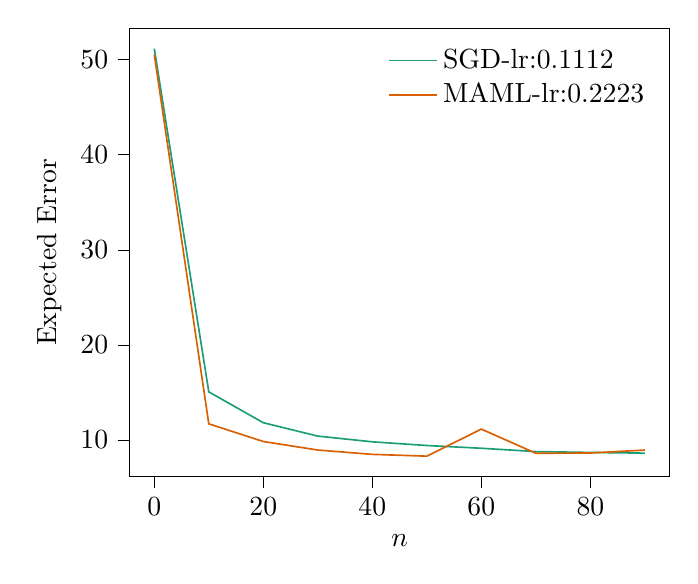
\begin{tikzpicture}

\definecolor{color0}{rgb}{0.105882352941176,0.619607843137255,0.466666666666667}
\definecolor{color1}{rgb}{0.850980392156863,0.372549019607843,0.00784313725490196}

\begin{axis}[
legend cell align={left},
legend style={fill opacity=0.8, draw opacity=1, text opacity=1, draw=none},
tick align=outside,
tick pos=left,
x grid style={white!69.0196078431373!black},
xlabel={\(\displaystyle n\)},
xmin=-4.5, xmax=94.5,
xtick style={color=black},
y grid style={white!69.0196078431373!black},
ylabel={Expected Error},
ymin=6.15067684345467, ymax=53.3020449055743,
ytick style={color=black}
]
\addplot [semithick, color0]
table {%
0 51.1588009027506
10 15.0551773772236
20 11.8102045684974
30 10.4024953768256
40 9.80259528491567
50 9.41420698541331
60 9.12405062147604
70 8.77346049993028
80 8.68396984937074
90 8.61166502038713
};
\addlegendentry{SGD-lr:0.1112}
\addplot [semithick, color1]
table {%
0 50.536439014682
10 11.6932479189217
20 9.83392703408676
30 8.93790927509903
40 8.4825370034006
50 8.29392084627828
60 11.138313244114
70 8.59982896840103
80 8.62491592814922
90 8.93725792162287
};
\addlegendentry{MAML-lr:0.2223}
\end{axis}

\end{tikzpicture}
